\chapter{Design}


\section{Vision}
\label{sec:vision}
Since the launcher had both a child-mode and a guardian-mode when we came with the initial design, this vision relies on the vision of the launcher project.\\ \\
	The initial idea of the WOMBAT system was a three-application tool to help educators illustrate time for the children they work with. One parts is the timer application as it is implemented, from which it is possible to run customized timers, such as an hourglass or a digital watch. This part should be available only from the guardian-mode.\\ \\
  The second part of the system is a timer overlay, which is launched when other applications, for example game applications, are launched through the GIRAF launcher. When such applications are launched through guardian mode, the user should be prompted to select if there is a time limit on the application, and what the limit should be. If a time limit is chosen, the given application, i.e. a game, is run with the timer overlay showing a custom timer with the time left.\\
	If the launcher is in child-mode, and the child opens some application, the timer overlay is run according to settings chosen in the third and last part of the WOMBAT system: the settings application. The overlay can be used if a child is only allowed to play a game for 30 minutes a day, then the overlay can be customized to show the child how long time is left of the allowed time. When the time is run out, the application is automatically closed.\\ \\
	The settings application is only available from the guardian-mode in the launcher, and from this application it is possible to customize which applications should be run with the timer overlay. Also it is possible to define how the overlay for every child should look like, and what should happen when the time limit has been reached. Also it is also possible to set constrains for the applications, such as time constrains, i.e. certain applications can only be opened in a different timespan on the day, or when a specific application has been run for 30 minutes straight, the application is closed and cannot be opened before a certain "cooldown" time.

\section{Use Cases}
A few use cases for each part of the vision.

\section{Paper Prototyping}
Paper prototypes\cite{misc:designInterSys} has been used in the first iterations in the development process. The initial idea of the system design was drawn on paper, so that our contact person, Mette als Andreasen, could give us some feedback on the design, before we started programming. Furthermore it made it easier for us to program, when there was a specific design to work towards. In figure \ref{fig:pap_prot_menu} is a paper prototype of the menu in the timer application, and the rest of the prototypes can be found in appendix \ref{sec:paper_prot}.

\begin{figure}[H]
	\centering
		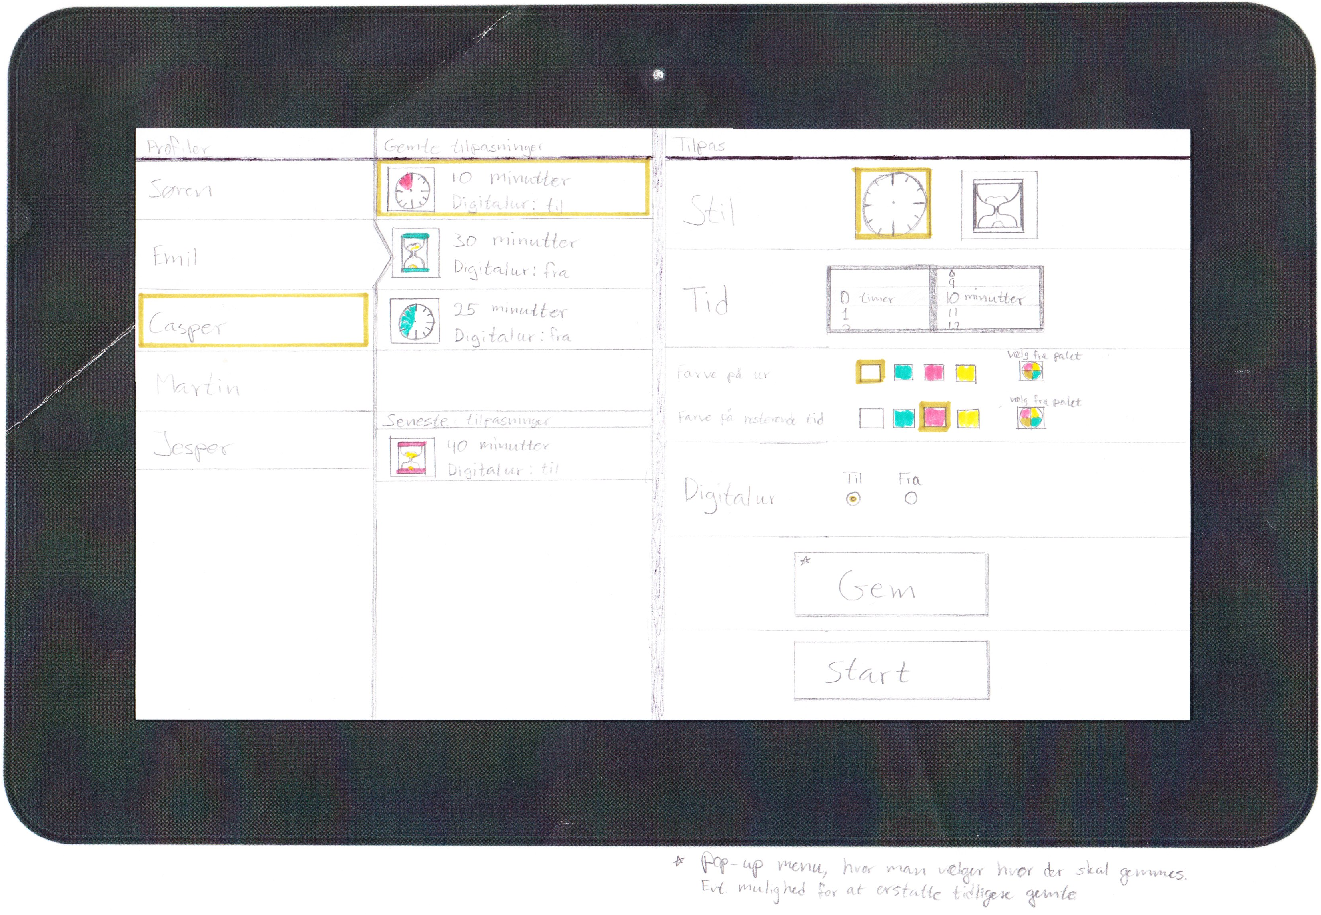
\includegraphics[width=\textwidth]{Images/paper_prototype/menu.png}
			\caption{Scan of a paper prototype of the menu in the timer application.}
	\label{fig:pap_prot_menu}
\end{figure}

Paper prototypes are produced quickly, and they capture early design ideas.

\subsection{Metaphors}
To enhance usability and learn-ability, we have used metaphors\cite{misc:designInterSys} on the buttons in the application. On the "Attach"-button, used to attach a second timer or one or two pictograms to the main timer, we have placed a paper-clip, which is known from the attach function in other programs, for example Microsoft Outlook Express. Furthermore we have used metaphors on the "Start Timer"-button, which looks like the "Play"-button known from various media players, and the "Save" and "Save As" buttons have a floppy disc icon, which is known from the save button in various word processing programs, for example Microsoft Office Word\footnote{Non-free word processor developed my Microsoft}. In figure \ref{fig:metaphors} examples of the implemented metaphors are shown along with screen-shots of other systems they are implemented in.

\begin{figure}[H]
	\centering
		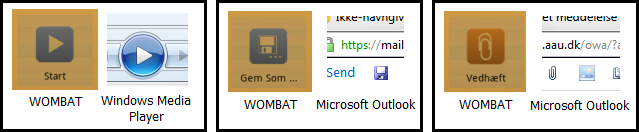
\includegraphics[width=\textwidth]{Images/Implementation/wombat_metaphors.png}
			\caption{Metaphors implemented in WOMBAT vs. original implementation.}
	\label{fig:metaphors}
\end{figure}